\section*{REFERENCES}

\def\refname{\vadjust{\vspace*{-1em}}} %Please don't do this in a real paper.

\subsubsection*{Basic format for books:}

\begin{thebibliography}{00}
\bibitem{b1} J. K. Author, ``Title of chapter in the book,'' in \textit{Title of His Published Book, x}th ed. City of Publisher,
(only U.S. State), Country: Abbrev. of Publisher, year, ch. x, sec. x, pp.
\textit{xxx--xxx.}
\end{thebibliography}

\subsubsection*{Examples:}

\begin{thebibliography}{00}
\bibitem{b2} G. O. Young, ``Synthetic structure of industrial
plastics,'' in \emph{Plastics}, 2nd ed., vol. 3, J. Peters, Ed. New York, NY, USA: McGraw-Hill, 1964, pp. 15--64.
\bibitem{b3} W.-K. Chen, \emph{Linear Networks and Systems}. Belmont, CA, USA: Wadsworth, 1993, pp. 123--135.
\end{thebibliography}

\subsubsection*{Basic format for periodicals:}

\begin{thebibliography}{00}
\bibitem{b4} J. K. Author, ``Name of paper,'' \textit{Abbrev. Title of Periodical}, vol. x, no. x, pp. xxx-xxx, Abbrev. Month, year, DOI.
10.1109.\textit{XXX}.123456.
\end{thebibliography}

\subsubsection*{Examples:}

\begin{thebibliography}{00}
\bibitem{b5} J. U. Duncombe, ``Infrared navigation---Part I: An
assessment of feasibility,'' \emph{IEEE Trans. Electron Devices}, vol. ED-11, no. 1, pp. 34--39, Jan. 1959, 10.1109/TED.2016.2628402.
\bibitem{b6} E. P. Wigner, ``Theory of traveling-wave optical laser,'' 
\emph{Phys. Rev.}, vol. 134, pp. A635--A646, Dec. 1965.
\bibitem{b7} E. H. Miller, ``A note on reflector arrays,'' \emph{IEEE
Trans. Antennas Propagat.}, to be published.
\bibitem{b8} H. Qin, Y. Cui, Z. Wu, Q. Chen and D. Xing, "Real-Time
Thermoacoustic Imaging-Guidance for Breast Tumor Resection," \emph{IEEE Photonics Journal}, vol. 12, no. 3, pp. 1--7, June 2020, Art no. 3700207.
\end{thebibliography}

\subsubsection*{Basic format for reports:}

\begin{thebibliography}{00}
\bibitem{b9} J. K. Author, ``Title of report,'' Abbrev. Name of Co., City of Co., Abbrev.
State, Country, Rep. {xxx}, year.
\end{thebibliography}

\subsubsection*{Examples:}

\begin{thebibliography}{00}
\bibitem{b10} E. E. Reber, R. L. Michell, and C. J. Carter, ``Oxygen absorption in the earth's atmosphere,'' Aerospace Corp., Los Angeles, CA, USA, Tech. Rep. TR-0200 (4230-46)-3, Nov. 1988.
\bibitem{b11} J. H. Davis and J. R. Cogdell, ``Calibration program for the 16-foot antenna,'' Elect. Eng. Res. Lab., Univ. Texas, Austin, TX, USA, Tech. Memo. NGL-006-69-3, Nov. 15, 1987.
\end{thebibliography}

\subsubsection*{Basic format for handbooks:}

\begin{thebibliography}{00}
\bibitem{b12} \textit{Name of Manual/Handbook}, x ed., Abbrev. Name of Co., City of Co., Abbrev. State, Country, year, pp.
\textit{xxx-xxx.}
\end{thebibliography}

\subsubsection*{Examples:}

\begin{thebibliography}{00}
\bibitem{b13} \textit{Transmission Systems for Communications}, 3rd ed., Western Electric Co., Winston-Salem, NC, USA, 1985, pp. 44--60.
\bibitem{b14} \textit{Motorola Semiconductor Data Manual}, Motorola Semiconductor Products Inc., Phoenix, AZ, USA, 1989.
\end{thebibliography}

\subsubsection*{Basic format for books (when available online): }

\begin{thebibliography}{00}
\bibitem{b15} J. K. Author, ``Title of chapter in the book,'' in \textit{Title of Published Book}, xth ed. City of
Publisher, State, Country: Abbrev. of Publisher, year, ch. x, sec. x, pp.
\textit{xxx--xxx}. [Online]. Available: \underline {http://www.web.com}. Accessed on: Month
Day, Year.
\end{thebibliography}

\subsubsection*{Examples:}

\begin{thebibliography}{00}
\bibitem{b16} G. O. Young, ``Synthetic structure of industrial
plastics,'' in \emph{Plastics}, vol. 3, Polymers of Hexadromicon, J.
Peters, Ed., 2nd ed. New York, NY, USA: McGraw-Hill, 1964, pp. 15--64.
[Online]. Available: \underline{http://www.bookref.com}. Accessed on: April 25, 2020.
\bibitem{b17} \textit{The Founders' Constitution}, Philip B. Kurland and Ralph Lerner, eds., Chicago, IL, USA: Univ. Chicago Press, 1987. [Online]. Available: \underline {http://press-pubs.uchicago.edu/founders/}. Accessed on: April 25, 2020.
\bibitem{b18} \emph{The Terahertz Wave eBook}. ZOmega Terahertz
Corp., 2014. [Online]. Available: \underline{http://dl.z-thz.com/eBook/zomega\_ebook\_pdf\_1206\_sr.pdf}. Accessed on: May 19, 2014.
\bibitem{b19} Philip B. Kurland and Ralph Lerner, eds., \textit{The
Founders' Constitution. }Chicago, IL, USA: Univ. of Chicago Press, 1987, [Online] Available: \emph{http://press-pubs.uchicago.edu/founders/}. Accessed on: Feb. 28, 2010.
\end{thebibliography}

\subsubsection*{Basic format for conference proceedings (published):}

\begin{thebibliography}{00}
\bibitem{b20} J. K. Author, ``Title of paper,'' in \textit{Abbreviated Name of Conf.}, City of Conf., Abbrev. State (if
given), Country, year, pp. \textit{xxxxxx.}
\end{thebibliography}

\subsubsection*{Example:}

\begin{thebibliography}{00}
\bibitem{b21} D. B. Payne and J. R. Stern, ``Wavelength-switched
passively coupled single-mode optical network,'' in \textit{Proc. IOOC-ECOC, }Boston, MA, USA, 1985,~pp.~585--590.
\end{thebibliography}

\subsubsection*{Basic format for papers presented at conferences when available online: }

\begin{thebibliography}{00}
\bibitem{b22} J.K. Author. (year, month). Title. presented at abbrev. conference title.
[Type of Medium]. Available: \underline{site/path/file}. Accessed on: Month Day, Year.
\end{thebibliography}

\subsubsection*{Example:}

\begin{thebibliography}{00}
\bibitem{b23} PROCESS Corporation, Boston, MA, USA. Intranets: Internet technologies deployed behind the firewall for corporate productivity. Presented at INET96 Annual Meeting. [Online]. Available: \underline {http://home.process.com/Intranets/wp2.htp}. Accessed on: April 25, 2020.
\end{thebibliography}

\subsubsection*{Basic format for reports and handbooks (when available online): }

\begin{thebibliography}{00}
\bibitem{b24} J. K. Author. ``Title of report,'' Company. City, State, Country. Rep. no.,
(optional: vol./issue), Date. [Online] Available:
\underline{site/path/file}. Accessed
on: Month Day, Year.
\end{thebibliography}

\subsubsection*{Examples:}

\begin{thebibliography}{00}
\bibitem{b25} R. J. Hijmans and J. van Etten, ``Raster: Geographic analysis and modeling with raster data,'' R Package Version 2.0-12, Jan. 12, 2012. [Online]. Available: \underline {http://CRAN.R-project.org/package=raster}. Accessed on: April 25, 2020.
\bibitem{b26} Teralyzer. Lytera UG, Kirchhain, Germany [Online]. Available: \emph{http://www.lytera.de/Terahertz\_THz\_Spectroscopy.php?id=home}, Accessed on: Jun. 5, 2014
\end{thebibliography}

\subsubsection*{Basic format for computer programs and electronic documents (when available online): }

\begin{thebibliography}{00}
\bibitem{b27} Legislative body. Number of Congress, Session. (year, month day). \textit{Number of bill or resolution}, \textit{Title}. [Type
of medium]. Available: \underline{site/path/file}
\end{thebibliography}

{\bfseries\itshape NOTE:} ISO recommends that capitalization follow the
accepted practice for the language or script in which the information is
given.

\subsubsection*{Example:}

\begin{thebibliography}{00}
\bibitem{b28} U.S. House. 102nd Congress, 1st Session. (1991, Jan. 11). \textit{H. Con. Res. 1, Sense of the Congress on Approval of Military Action}. [Online]. Available: LEXIS Library: GENFED File: BILLS
\end{thebibliography}

\subsubsection*{Basic format for patents (when available online):}

\begin{thebibliography}{00}
\bibitem{b29} Name of the invention, by inventor's name. (year, month day). Patent Number [Type
of medium]. Available: \underline{site/path/file}
\end{thebibliography}

\subsubsection*{Example:}

\begin{thebibliography}{00}
\bibitem{b30} Musical toothbrush with mirror, by L.M.R. Brooks. (1992, May 19). Patent D 326 189 [Online]. Available: NEXIS Library: LEXPAT File: DES
\end{thebibliography}

\subsubsection*{Example for papers presented at conferences (unpublished):}

\begin{thebibliography}{00}
\bibitem{b31} D. Ebehard and E. Voges, ``Digital single sideband
detection for interferometric sensors,'' presented at the \textit{2nd Int. Conf. Optical Fiber Sensors,} Stuttgart, Germany, Jan. 2--5, 1984.
\end{thebibliography}

\subsubsection*{Basic format for patents:}

\begin{thebibliography}{00}
\bibitem{b32} J. K. Author, ``Title of patent,'' U.S. Patent {x xxx xxx}, Abbrev. Month, day, year.
\end{thebibliography}

\subsubsection*{Example:}

\begin{thebibliography}{00}
\bibitem{b33} G. Brandli and M. Dick, ``Alternating current fed power supply,'' U.S. Patent 4 084 217, Nov. 4, 1978.
\end{thebibliography}

\subsubsection*{Basic format for theses (M.S.) and dissertations (Ph.D.):}

\begin{thebibliography}{00}
\bibitem{b34} J. K. Author, ``Title of thesis,'' M.S. thesis, Abbrev. Dept., Abbrev.
Univ., City of Univ., Abbrev. State, year. p. nnn.
\bibitem{b35} J. K. Author, ``Title of dissertation,'' Ph.D. dissertation, Abbrev.
Dept., Abbrev. Univ., City of Univ., Abbrev. State, year. p. nnn.
\end{thebibliography}

\subsubsection*{Examples:}

\begin{thebibliography}{00}
\bibitem{b36} J. O. Williams, ``Narrow-band analyzer,'' Ph.D. dissertation, Dept. Elect. Eng., Harvard Univ., Cambridge, MA, USA, 1993. p. 50.
\bibitem{b37} N. Kawasaki, ``Parametric study of thermal and chemical nonequilibrium nozzle flow,'' M.S. thesis, Dept. Electron. Eng., Osaka Univ., Osaka, Japan, 1993. p. 30.
\end{thebibliography}

\subsubsection*{Basic format for the most common types of unpublished references:}

\begin{thebibliography}{00}
\bibitem{b38} J. K. Author, private communication, Abbrev. Month, year.
\bibitem{b39} J. K. Author, ``Title of paper,'' unpublished.
\bibitem{b40} J. K. Author, ``Title of paper,'' to be published.
\end{thebibliography}

\subsubsection*{Examples:}

\begin{thebibliography}{00}
\bibitem{b41} A. Harrison, private communication, May 1995.
\bibitem{b42} B. Smith, ``An approach to graphs of linear forms,'' unpublished.
\bibitem{b43} A. Brahms, ``Representation error for real numbers in binary computer arithmetic,'' IEEE Computer Group Repository, Paper R-67-85.
\end{thebibliography}

\subsubsection*{Basic formats for standards:}

\begin{thebibliography}{00}
\bibitem{b44} \textit{Title of Standard}, Standard number, date.
\bibitem{b45} \textit{Title of Standard}, Standard number, Corporate author, location, date.
\end{thebibliography}

\subsubsection*{Examples:}

\begin{thebibliography}{00}
\bibitem{b46} \emph{IEEE Criteria for Class IE Electric Systems}, IEEE Standard 308, 1969.
\bibitem{b47} \emph{Letter Symbols for Quantities}, ANSI Standard Y10.5-1968.
\end{thebibliography}

\subsubsection*{Article number in~reference examples:}

\begin{thebibliography}{00}
\bibitem{b48} R. Fardel, M. Nagel, F. Nuesch, T. Lippert, and A. Wokaun, ``Fabrication of organic light emitting diode pixels by laser-assisted forward transfer,'' \textit{Appl. Phys. Lett.}, vol. 91, no. 6, Aug. 2007, Art. no. 061103.
\bibitem{b49} J. Zhang and N. Tansu, ``Optical gain and laser characteristics of InGaN quantum wells on ternary InGaN substrates,'' \textit{IEEE Photon. J.}, vol. 5, no. 2, Apr. 2013, Art. no. 2600111
\end{thebibliography}

\subsubsection*{Example when using et al.:}

\begin{thebibliography}{00}
\bibitem{b50} S. Azodolmolky, Jordi Perell\'{o}, Marianna Angelou, Fernando Agraz, Luis Velasco, Salvatore Spadaro,~\textit{et al.}, Experimental demonstration of an impairment aware network planning and operation tool for transparent/translucent optical networks,''~\textit{J. Lightwave. Technol.}, vol. 29, no. 4, pp. 439--448, Sep. 2011.
\end{thebibliography}

\begin{IEEEbiography}[{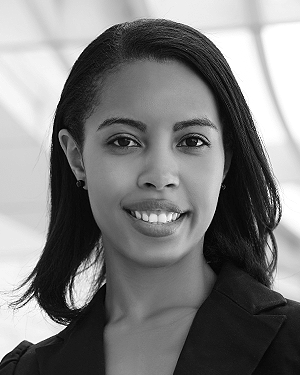
\includegraphics[width=1in,height=1.25in,clip,keepaspectratio]{a1.png}}]{FIRST
A. AUTHOR } (Fellow, IEEE) and all authors may include 
biographies. Biographies are often not included in conference-related
papers. This author became a Member (M) of IEEE in 1976, a Senior
Member (SM) in 1981, and a Fellow (F) in 1987. The first paragraph may
contain a place and/or date of birth (list place, then date). Next,
the author's educational background is listed. The degrees should be
listed with type of degree in what field, which institution, city,
state, and country, and year the degree was earned. The author's major
field of study should be lower-cased. 

The second paragraph uses the pronoun of the person (he or she) and not the 
author's last name. It lists military and work experience, including summer 
and fellowship jobs. Job titles are capitalized. The current job must have a 
location; previous positions may be listed 
without one. Information concerning previous publications may be included. 
Try not to list more than three books or published articles. The format for 
listing publishers of a book within the biography is: title of book 
(publisher name, year) similar to a reference. Current and previous research 
interests end the paragraph. The third paragraph begins with the author's 
title and last name (e.g., Dr.\ Smith, Prof.\ Jones, Mr.\ Kajor, Ms.\ Hunter). 
List any memberships in professional societies other than the IEEE. Finally, 
list any awards and work for IEEE committees and publications. If a 
photograph is provided, it should be of good quality, and 
professional-looking. Following are two examples of an author's biography.
\end{IEEEbiography}

\begin{IEEEbiography}[{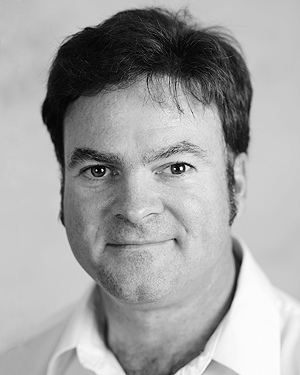
\includegraphics[width=1in,height=1.25in,clip,keepaspectratio]{a2.png}}]{SECOND
B. AUTHOR } was born in Greenwich Village, New York, NY, USA in 
1977. He received the B.S. and M.S. degrees in aerospace engineering from 
the University of Virginia, Charlottesville, in 2001 and the Ph.D. degree in 
mechanical engineering from Drexel University, Philadelphia, PA, in 2008.

From 2001 to 2004, he was a Research Assistant with the Princeton Plasma 
Physics Laboratory. Since 2009, he has been an Assistant Professor with the 
Mechanical Engineering Department, Texas A{\&}M University, College Station. 
He is the author of three books, more than 150 articles, and more than 70 
inventions. His research interests include high-pressure and high-density 
nonthermal plasma discharge processes and applications, microscale plasma 
discharges, discharges in liquids, spectroscopic diagnostics, plasma 
propulsion, and innovation plasma applications. He is an Associate Editor of 
the journal \emph{Earth, Moon, Planets}, and holds two patents. 

Dr. Author was a recipient of the International Association of Geomagnetism 
and Aeronomy Young Scientist Award for Excellence in 2008, and the IEEE 
Electromagnetic Compatibility Society Best Symposium Paper Award in 2011. 
\end{IEEEbiography}

\begin{IEEEbiography}[{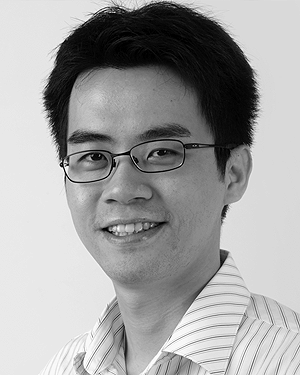
\includegraphics[width=1in,height=1.25in,clip,keepaspectratio]{a3.png}}]{THIRD
C. AUTHOR,~JR. } (Member, IEEE) received the B.S. degree in mechanical 
engineering from National Chung Cheng University, Chiayi, Taiwan, in 2004 
and the M.S. degree in mechanical engineering from National Tsing Hua 
University, Hsinchu, Taiwan, in 2006. He is currently pursuing the Ph.D. 
degree in mechanical engineering at Texas A{\&}M University, College 
Station, TX, USA.

From 2008 to 2009, he was a Research Assistant with the Institute of 
Physics, Academia Sinica, Tapei, Taiwan. His research interest includes the 
development of surface processing and biological/medical treatment 
techniques using nonthermal atmospheric pressure plasmas, fundamental study 
of plasma sources, and fabrication of micro- or nanostructured surfaces. 

Mr. Author's awards and honors include the Frew Fellowship (Australian 
Academy of Science), the I. I. Rabi Prize (APS), the European Frequency and 
Time Forum Award, the Carl Zeiss Research Award, the William F. Meggers 
Award and the Adolph Lomb Medal (OSA).
\end{IEEEbiography}